\documentclass{article}
\usepackage[a4paper, margin=1in]{geometry}
\usepackage[utf8]{inputenc}
\usepackage[russian]{babel}
\usepackage{wrapfig}
\usepackage{graphicx}
\usepackage{amsmath}
\usepackage{amssymb}
\usepackage{float}
\usepackage{url}

\graphicspath{{./images/}}


\title{Математические методы в робототехнике}
\author{Чистый Аркадий\\
Хохлов Николай\\
Молчанов Егор\\
Научный руководитель: Мисюрин Сергей Юрьевич}
\date{May 2021}

\begin{document}
\begin{center}
МИНИСТЕРСТВО НАУКИ И ВЫСШЕГО ОБРАЗОВАНИЯ РОССИЙСКОЙ ФЕДЕРАЦИИ
\vfill
Федеральное государственное автономное образовательное учреждение высшего образования

\bigskip
Национальный исследовательский ядерный университет «МИФИ»
\vfill
ИНСТИТУТ ИНТЕЛЛЕКТУАЛЬНЫХ КИБЕРНЕТИЧЕСКИХ СИСТЕМ
\vfill
Направление подготовки: 01.03.02 Прикладная математика и информатика
\vfill
ПРОЕКТНАЯ ПРАКТИКА
\vfill
{\large Пояснительная записка к проекту

\medskip
{\bfseries \Large <<Математические методы в робототехнике>>}}
\vfill
\end{center}
\begin{flushright}
Выполнили:\\Чистый Аркадий, Б19-511 \\Хохлов Николай, Б19-501\\Молчанов Егор, Б19-501\\
\medskip
Научный руководитель:\\ Мисюрин Сергей Юрьевич
\end{flushright}
\vfill
\vfill
\begin{center}
Москва, 23 мая 2021 года
\end{center}
\vfill
\vfill
\pagebreak

\tableofcontents
\newpage

\section{Введение}
В настоящее время разработка и производство шестиногих шагающих роботов (роботов-пауков) является одним из приоритетных научно-технических направлений. Шестиногие роботы устойчивее двуногих или зооморфных роботов за счет его количества ног \cite{ref1}. Такие роботы обладают повышенной устойчивостью, наиболее эффективны в условиях бездорожья, сложного рельефа и при преодолении препятствий – даже на вязких грунтах они могут быть эффективнее механизмов с гусеничными движителями \cite{ref2,ref3}, традиционно считающихся наиболее проходимыми. Таким образом увеличение скорости и эффективности передвижения шагающих роботов является актуальным направлением исследований. По результатам деятельности прошлого семестра, мы определили оптимальный алгоритм передвжения механизма, поэтому в этом семестре мы исследовали возможности оптимизации различных составляющих робота.
\newpage
\section{Постановка задачи}
Основная цель - оптимизация отдельных компонент робота-паука, влияющих на эффективность передвижения.

Существенным элементом, отвечающим за это является нога робота. Следовательно, требуется построить математическую модель ноги паука, позволяющую проводить исследования этого механизма с целью дальнейшей оптимизации.
Наряду с ногой паука, важнейшим звеном в управлении являются двигатели (сервоприводы) робота. Необходимо изучить разные варианты подключения двигателей, их режимы работы, а также их взаимодействие с программным обеспечением, управляющим роботом.
\newpage

\section{Управление двигателями}
Скорость передвижения пространственного механизма напрямую зависит от скорости движения его отдельных компонент. Поэтому, важно добиться максимальной скорости поворота сервоприводов.

Для оптимизации движения отдельных двигателей необходимо понять, на что тратится и как распределяется время при повороте двигателя. Для этого нужно изучить протокол передачи данных между управляющей частью механизма и приводами.

В открытом доступе \cite{ref9} был найден протокол управления двигателем (см. табл. \ref{tab:protocol}), подобном тому, который установлен на лабораторном роботе-пауке. В исходном коде поставляемой с роботом библиотеке были найдены похожие команды, был сделан вывод, что изложенный в источнике протокол полностью или частично описывает управление двигателем лабороторной модели.

\begin{table}[h]
\centering
\begin{tabular}{|c|c|}
    \hline
    Описание & Пример \\
    \hline \hline
    Заголовок & 0x55 0x55 \\ \hline
    ID привода & 9 \\ \hline
    Размер данных & 7 \\ \hline
    Команда & 1 \\ \hline
    Параметры & 0x10 0x15 \\ \hline
    Контрольная сумма & 0x5f \\  \hline
\end{tabular}
\caption{Протокол управления приводом}
\label{tab:protocol}
\end{table}

Исходная библиотека для управления приводами написана на Python. Python - относительно медленный язык программирования, поэтому было принято решение переписать библиотеку на более быстрый язык программирования. В качестве такого языка был выбран C.

После переписывания библиотеки сравнивалось времени записи одной команды записи (т.е. поворота двигателя на заданный угол) на основе двух библиотек: исходной и переписанной. Среднее время записи  вычислялось как среднее арифметическое следующим образом:
\[t = \frac{T}{N},\] где $T$ -- общее время записи $N$ команд последовательно, $N$ -- количество команд.

Результаты эксперимента представлены в табл. \ref{tab:compar1}. Как видно из таблицы, существенных изменений в скорости записи нет. Для удобства работы дальнейшие измерения и манипуляции будут производиться с языком Python.

\begin{table}[h]
\centering
\begin{tabular}{|c|c|}
    \hline
    Язык программирования & Время записи \\
    \hline \hline
    Python & 0.31 мс \\
    \hline
    C++ & 0.29 мс \\
    \hline
\end{tabular}
\caption{Время записи на основе разных библиотек}
\label{tab:compar1}
\end{table}

Для того, чтобы создать алгоритм, который динамически управляет двигателем, необходим постоянный обмен информацией с двигателем, а именно опрос его текущего положения и корректировка скорости.

Необходимо было произвести измерение скорости записи и чтения информации. А также измерялось время попеременно выполняющихся команд чтения и записи. 

\begin{table}[h]
\centering
\begin{tabular}{|c|c|c|}
    \hline
    Время записи & Время чтения & Время чтения и записи \\
    \hline \hline
    0.31 мс & 10 мс & 10-300 мс \\
    \hline
\end{tabular}
\caption{Время выполнения команд}
\label{tab:compar2}
\end{table}

Как можно видеть из табл. \ref{tab:compar2}, чтение происходит достаточно медленно и занимает намного больше времени чем запись. Попеременно выполняющиеся команды чтения и записи выполняются ещё медленнее и время выполнения варьируется в широком диапазоне от 30 до 300 мс.

\newpage

\section{Математическая модель ноги робота}

\subsection{Геометричесая модель ноги робота}

\begin{figure}[h]
\centering
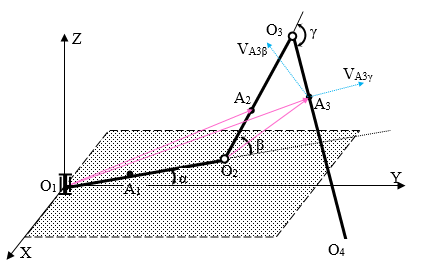
\includegraphics[height=12em]{images/leg_skhem.png}
\caption{Модель ноги робота-паука}
\label{fig:leg_model}
\end{figure}

Рассмотрим модель ноги нашего робота (см. рис. \ref{fig:leg_model}). Нога состоит из трех звеньев (\emph{tibia}, \emph{femur}, \emph{coxa}). Обозначим концы звеньев точками $O_1, O_2, O_3, O_4,$ а их центры масс точками $A_1, A_2, A_3, $ как показано на рисунке. Ясно, что данная система имеет ровно 3 степени свободы, поэтому для полного описания состояния этой механической системы требуется ввести три обобщенные координаты: $\alpha$ --- угол между звеном \emph{tibia} и осью $O_1Y$, $\beta$ --- угол между звеном \emph{femur} и осью $O_1O_2$, $\gamma$ --- угол между звеном \emph{coxa} и осью $O_2O_3$.

Введем обозначения для длин звеньев:
\begin{align*}
|O_1O_2| &= l_1, & |O_1A_1| &= \rho_1, & |O_1A_2| &= L_1,\\
|O_2O_3| &= l_2, & |O_2A_2| &= \rho_2, & |O_1A_3| &= L_2,\\
|O_3O_4| &= l_3, & |O_3A_3| &= \rho_3, & |O_2A_3| &= L_3;
\end{align*}

$m_1, m_2, m_3$ - массы звеньев, $J_{A_1}, J_{A_2},J_{A_3}$ - моменты инерции звеньев относительно центров масс.

\subsection{Уравнение Лагранжа второго рода}

Если голономная механическая система (система, механические связи которой можно свести к геометрическим) описывается лагранжианом $L(q_{i},{\dot {q}_{i}},t)$, где $q_{i}$ --- обобщённые координаты, $t$ --- время, точкой обозначено дифференцирование по времени) и в системе действуют только потенциальные силы, то уравнения Лагранжа второго рода имеют вид  \[{\frac {d}{dt}}\left({\frac {\partial L}{\partial {\dot {q}}_{i}}}\right)-{\frac {\partial L}{\partial q_{i}}}=0,\] где $i = 1,2,\ldots,n$ ($n$ -- число степеней свободы механической системы). Лагранжиан представляет собой разность кинетической и потенциальной энергий системы \cite{ref4}.
При наличии и потенциальных, и непотенциальных обобщённых сил появляется правая часть: \[\frac{d}{dt} \left( \frac{\partial L}{\partial\dot q_i} \right) - \frac{\partial L}{\partial q_i} = R_i .\]

Составим функцию лагранжиана для исследуемой системы. Согласно определению имеем:
\[L = T_1 + T_2 + T_3 - U_2 - U_3,\] где $T_1, T_2, T_3$ и $U_2, U_3$ - функции кинетической и потенциальной энергии звеньев соответственно. Для них имеют место равенства:

\begin{align*}
T_1 &= \frac{1}{2} (m_1\rho_1^2 + J_{A_1} + J_{g_1}) \dot\alpha^2,\\
T_2 &= \frac{m_2}{2}(L_1^2\dot\alpha^2+\rho_2^2\dot\beta^2) + \frac{J_{A_2}}{2}((\dot\alpha\cos{\beta})^2+\dot\beta^2) + \frac{J_{g_2}}{2}\dot\beta^2,\\
T_3 &= \frac{m_3}{2}(L_2^2\dot\alpha^2+L_3^2\dot\beta^2+\rho_3^2\dot\gamma^2+(L_3^2+\rho_3^2-l_2^2)\dot\beta\dot\gamma) + \frac{J_{A_3}}{2}((\dot\alpha\cos{(\gamma - \beta)})^2 + (\dot\gamma-\dot\beta)^2) + \frac{J_{g_3}}{2}\dot\gamma^2,\\
U_2 &= m_2g\rho_2\sin{\beta} + m_{g_3}gl_2\sin{\beta},\\
U_3 &= m_3gl_2\sin{\beta}-m_3g\rho_3\sin{(\gamma-\beta)}.
\end{align*}

Подставив полученные равенства в выражение для лагранжиана, воспользуемся уравнениями Эйлера-Лагранжа второго рода. В результате после дифференцирования лагранжиана мы можем получить нормальную систему обыкновенных дифференциальных уравнений второго порядка:
\begin{align*}
\begin{cases}
\ddot\alpha &= f_1(\alpha,\beta,\gamma,\dot\alpha,\dot\beta,\dot\gamma)\\
\ddot\beta &= f_2(\alpha,\beta,\gamma,\dot\alpha,\dot\beta,\dot\gamma)\\
\ddot\gamma &= f_3(\alpha,\beta,\gamma,\dot\alpha,\dot\beta,\dot\gamma)
\end{cases}
\end{align*}

Функции $f_1, f_2, f_3$ являются известными аналитическими функциями, которые можно выразить явно, однако выражения для их записи являются слишком громоздкими, поэтому в данном случае оставим их в такой записи.

\subsection{Методы Рунге-Кутты}
Методы Рунге-Кутты --- обширный класс численных методов, применяемых для решения задачи Коши для обыкновенных дифференциальных уравнений и их систем. Первые методы данного класса были предложены около 1900 года немецкими математиками К. Рунге и М. В. Куттой. 

К классу методов Рунге — Кутты относятся явный метод Эйлера и модифицированный метод Эйлера с пересчётом, которые представляют собой соответственно методы первого и второго порядка точности. Существуют стандартные явные методы третьего порядка точности, не получившие широкого распространения. Наиболее часто используется и реализован в различных математических пакетах классический метод Рунге — Кутты, имеющий четвёртый порядок точности. При выполнении расчётов с повышенной точностью всё чаще применяются методы пятого и шестого порядков точности \cite{ref5,ref6}. Построение схем более высокого порядка сопряжено с большими вычислительными трудностями \cite{ref7}. Методы седьмого порядка должны иметь по меньшей мере девять стадий, а методы восьмого порядка — не менее 11 стадий. Для методов девятого и более высоких порядков (не имеющих, впрочем, большой практической значимости) неизвестно, сколько стадий необходимо для достижения соответствующего порядка точности \cite{ref7}.

Для решения полученной нами системы мы использовали стандартный метод Рунге-Кутты четвертого порядка. Из всего семейства данных числовых методов мы выбрали именно его, потому что данный метод позволяет получать решения с достаточно высокой точностью, при этом объем требуемых вычислений остается небольшим в сравнении с методами высших порядков. Разберем подробнее основную идею этого метода.

Рассмотрим задачу Коши для системы обыкновенных дифференциальных уравнений первого порядка. Всюду далее $\boldsymbol{y}, \boldsymbol{f},\boldsymbol{k_i} \in \mathbb{R}^n,$ а $t,h \in \mathbb{R}.$

\begin{align*}
\frac{d\boldsymbol{y}}{dt} &= \boldsymbol{f}(t,\boldsymbol{y})\\
\boldsymbol{y}(t_0) &= \boldsymbol{y_0},
\end{align*}

Здесь $\boldsymbol{y}$ --- неизвестная вектор-функция времени $t$, которую мы будем стараться аппроксимировать. В начальный момент времени $t_0$ соответствующее значение $\boldsymbol{y} = \boldsymbol{y_0}.$ Функция $\boldsymbol{f}$ и начальные условия $t_0, \boldsymbol{y_0}$ считаются данными.

Далее введем величину размера шага $h > 0$ и определим
\begin{align*}
\boldsymbol{y}_{n+1} &= \boldsymbol{y}_n + \frac{h}{6}(\boldsymbol{k_1} + 2\boldsymbol{k_2} + 2\boldsymbol{k_3} + \boldsymbol{k_4})\\
t_{n+1} &= t_n + h,
\end{align*}
где $n = 0,1,2 \ldots$ 

\begin{figure}[h]
\centering
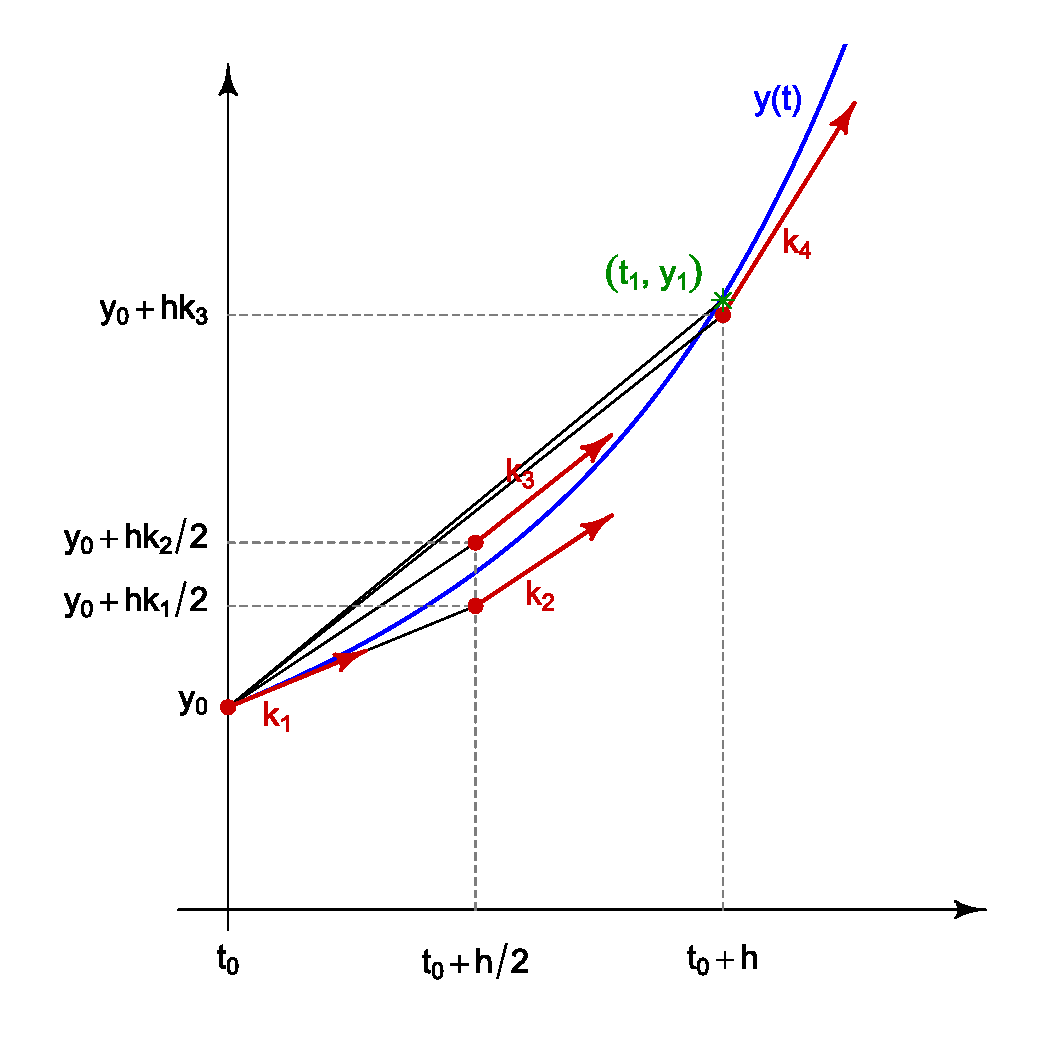
\includegraphics[width=20em,height=20em]{images/runge-kutta_slopes.pdf}
\caption{Аппроксимация функции в методе Рунге-Кутты \cite{ref8}}
\label{fig:runge-kutta}
\end{figure} 
Выражения для $\boldsymbol{k_1},\boldsymbol{k_2},\boldsymbol{k_3},\boldsymbol{k_4}$ выглядят следующим образом: 

\begin{align*}
\boldsymbol{k_1} &= \boldsymbol{f}(t_n,\boldsymbol{y}_n),\\
\boldsymbol{k_2} &= \boldsymbol{f}(t_n + \frac{h}{2}, \boldsymbol{y}_n + \frac{h}{2}\boldsymbol{k_1}),\\
\boldsymbol{k_3} &= \boldsymbol{f}(t_n + \frac{h}{2}, \boldsymbol{y}_n + \frac{h}{2}\boldsymbol{k_2}),\\
\boldsymbol{k_4} &= \boldsymbol{f}(t_n + h,\boldsymbol{y}_n+h\boldsymbol{k_3}).
\end{align*}

Как видно из рис. \ref{fig:runge-kutta}, $y_{n+1}$ --- это приближенное значение выражения $y(t_{n+1})$, последующие значения $y_{n+1}$ определяются предыдущем значением $y_{n}$ и средним значением четырех инкрементов. Каждый из инкрементов является произведением величины $h$ на тангенс угла наклона касательной $\boldsymbol{k_i}$, задаваемый функцией $\boldsymbol{f}$, стоящей в правой части системы.  

\begin{itemize}
    \item $\boldsymbol{k_1}$ --- это наклон функции в начале интервале
    \item $\boldsymbol{k_2}$ --- это наклон функции в середине интервала (используя $\boldsymbol{y}$ и $\boldsymbol{k_1})$
    \item $\boldsymbol{k_3}$ --- это наклон функции в середине интервала (используя $\boldsymbol{y}$ и $\boldsymbol{k_2}$)
    \item $\boldsymbol{k_4}$ --- это наклон функции в конце интервала
\end{itemize}

Этот метод имеет четвертый порядок точности, это означает, что ошибка на одном на шаге равна $O$($h^5$), а суммарная ошибка на конечном интервале имеет порядок $O$($h^4$).

Чтобы решить систему дифференциальных уравнений, описывающую механические связи между всеми звеньями ноги, нами был разработан и реализован программный комплекс, который позволяет численно решать достаточно произвольные системы дифференциальных уравнений. В качестве языка программирования для реализации использовался язык C\texttt{++}. Этому способствовал ряд причин. Во-первых, выбранный язык должен был обладать большой безопасностью. Во-вторых, нужна была возможность писать обобщенный код (что реализовано в C\texttt{++} с помощью шаблонов). В-третьих, C\texttt{++} сильно уменьшает сложность кода за счет перегрузки функций и операторов (требовалось для реализации операций над вектор-функциями). В-четвертых, C\texttt{++} имеет достаточно большую скорость вычислений, необходимую для эффективной работы метода Рунге-Кутты.

Наконец, для решения системы нам нужно было знать значения различных геометрических и физических параметров реального робота-паука (длины звеньев ног, координаты их центров масс, значения моментов инерции звеньев и др.). Поэтому нами были произведены измерения перечисленных выше параметров робота. Далее мы ввели численные значения этих параметров и явные выражения для правой части системы дифференциальных уравнений (функции $f_1, f_2, f_3$) в программу. В итоге мы получили численные зависимости трех обобщенных координат (и их производных) от времени, при свободном движении ноги.

\begin{figure}[H]
\centering
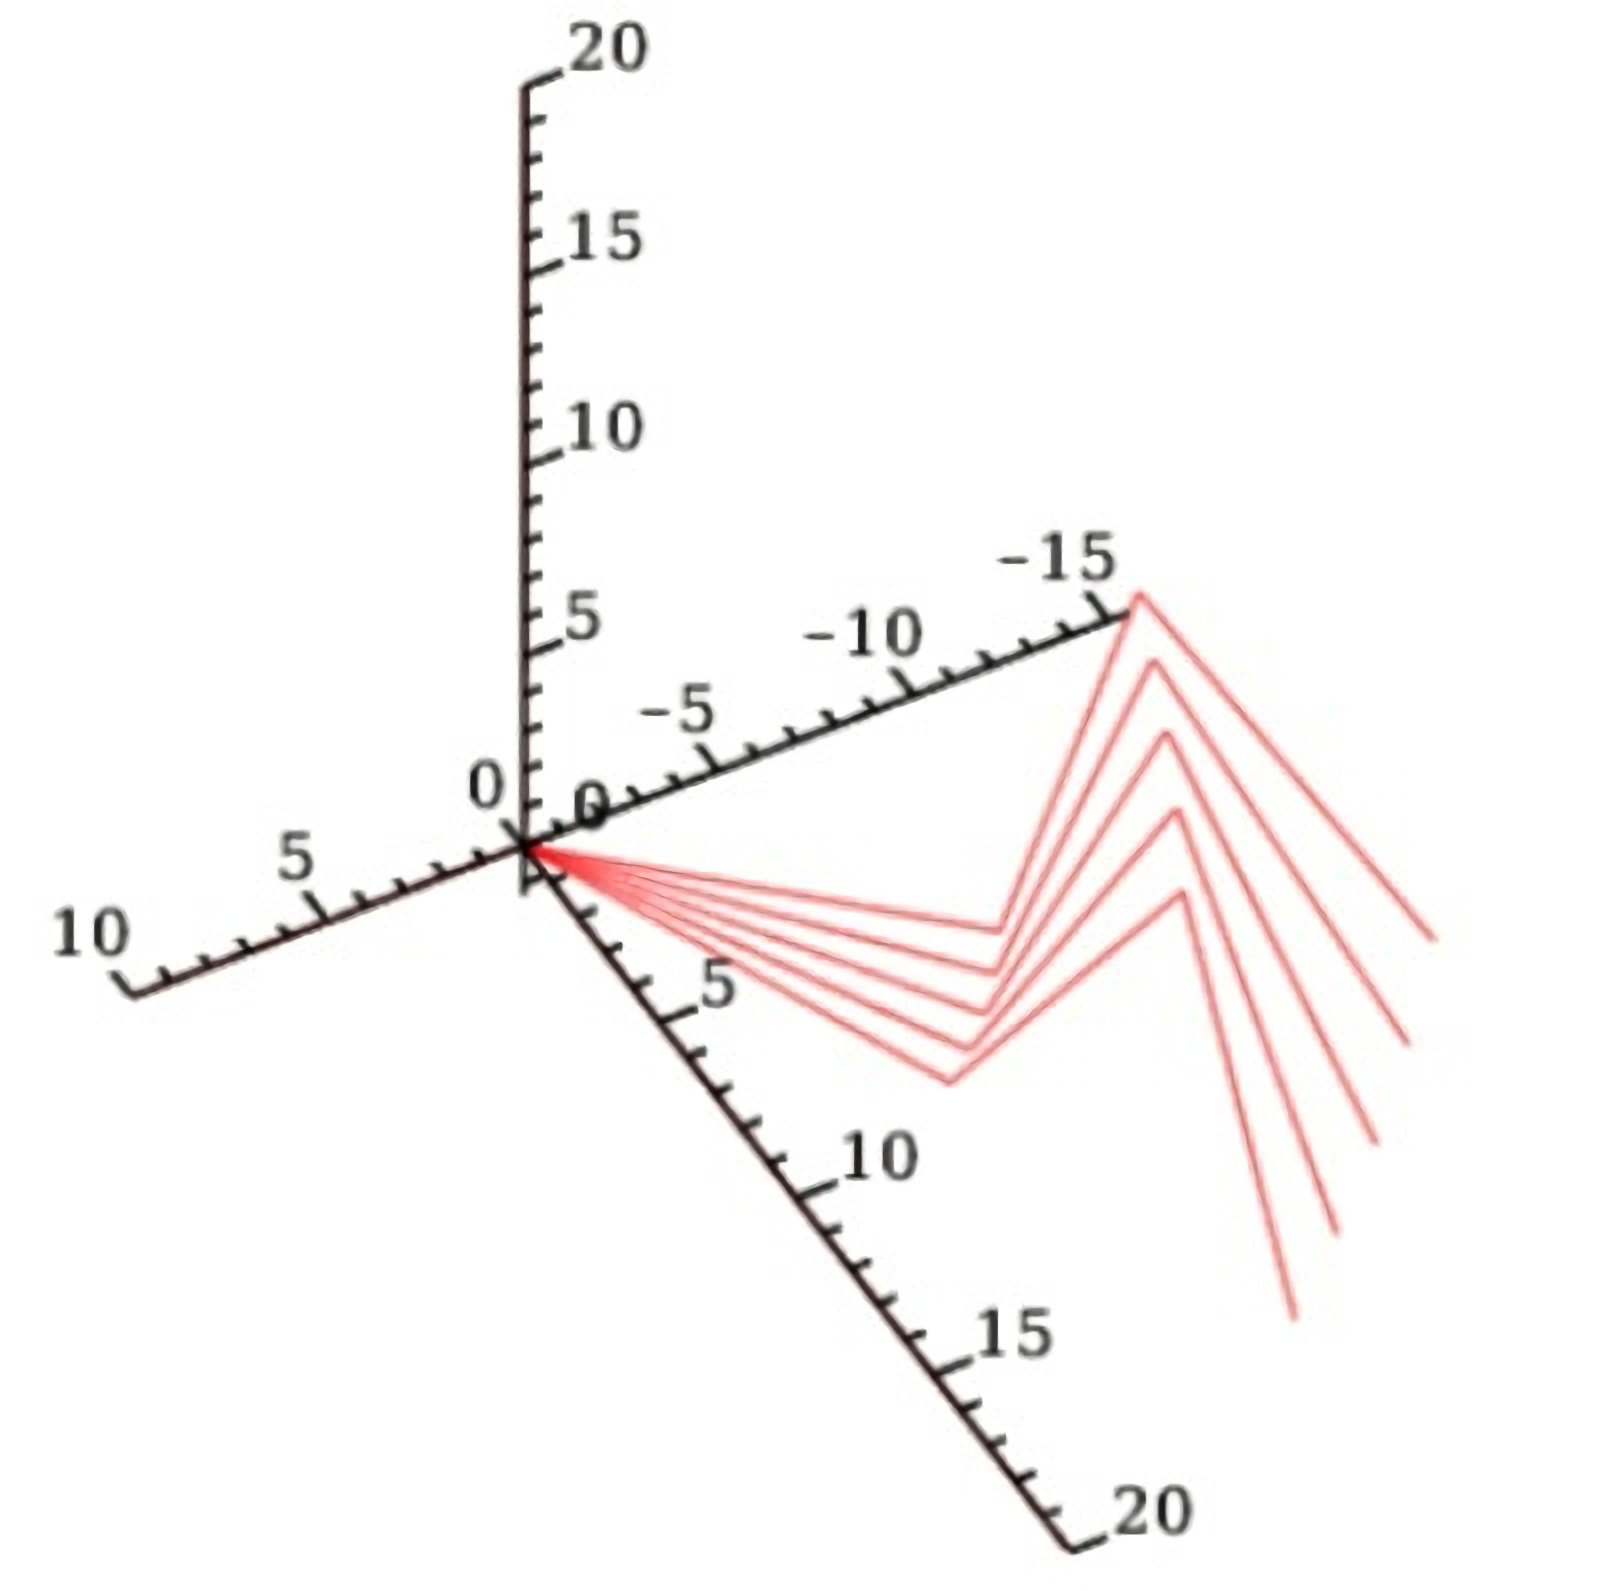
\includegraphics[height=10em]{images/leg_modeling.jpg}
\caption{Моделирование движения ноги робота-паука}
\label{fig:leg_modeling}
\end{figure}

Для наглядной иллюстрации была написана программа для изображения ноги робота-паука в заданный момент времени (на рис. \ref{fig:leg_modeling} изображены пять последовательных изображений ноги робота с шагом в 0.2 секунды). Данные для определения положения ноги брались из полученного ранее численного решения системы уравнений. Таким образом, мы смогли смоделировать свободное движение ноги в отсутствии непотенциальных сил.

\newpage

\begin{thebibliography}{9}
\bibitem{ref9}
LX-15D Bus Servo [Электронный ресурс]: Dropbox. --
\\
\url{https://www.dropbox.com/sh/b3v81sb9nwir16q/AADXOwhdw7KLq5t5UM8ND3kwa/LX-15D%20Bus%20Servo?dl=0&subfolder_nav_tracking=1}

\bibitem{ref1}
Kim J.Y., Yang U.J. Mechanical design of powered prosthetic leg and walking pattern generation based on motion capture data. Advanced Robotics. 2015. vol. 29. no. 16. Р. 1061–1079.

\bibitem{ref2}
Hong S., Kim H.W., Choi J.S. Transient Dynamic Analysis of Tracked Vehicles on Extremely Soft Cohesive soil, The 5th ISOPE Pacific/Asia Offshore Mechanics Symposium, 2002, pp. 100-107.

\bibitem{ref3}
Briskin E.S., Chernyshev V.V., Maloletov A.V., Sharonov N.G. Sravnitel'nyy analiz kolesnykh, gusenichnykh i shagayushchikh mashin [Comparative analysis of wheeled, tracked and walking machines], Robototekhnika i tekhnicheskaya kibernetika [Robotics and Technical Cybernetics], 2013, No. 1, pp. 6-14.

\bibitem{ref4}
Ландау Л. Д., Лифшиц Е. М. Теоретическая физика: Учеб. пособие. -- В 10-ти т. Т. І. Механика. -- 4-е изд., испр. -- М.: Наука. Гл. ред. физ.-мат. лит., 1988, C. 9-17.

\bibitem{ref5}
Бахвалов Н. С., Жидков Н. П., Кобельков Г. М. . Численные методы. -- М.: Лаборатория Базовых Знаний, 2001. -- 630 с. -- ISBN 5-93208-043-4. -- С. 363—375.

\bibitem{ref6}
Ильина В. А., Силаев П. К. . Численные методы для физиков-теоретиков. Ч. 2. -- Москва-Ижевск: Институт компьютерных исследований, 2004. -- 118 с. -- ISBN 5-93972-320-9. -- С. 16-30.

\bibitem{ref7}
Butcher J. C.[en] . Numerical Methods for Ordinary Differential Equations. -- New York: John Wiley and Sons, 2008. -- ISBN 978-0-470-72335-7.

\bibitem{ref8}
Runge–Kutta methods [Электронный ресурс]: Wikipedia. The Free Encyclopedia. –- URL: \\
\url{https://en.wikipedia.org/wiki/Runge%E2%80%93Kutta_methods}.


\end{thebibliography}

\end{document}
